%!TEX root =  bgo-cam-ready.tex
% please do not delete or change the first line (needed by Csaba's editor)
%%%%%%%%%%%%%%%%%%%%%%%%%%%%%%%%%%%%%%%%%%%%%%%%%%%%%%%%%%%%%%%%%%%%%%%%%%%%%%% 
\subsection{Proof of Theorem \ref{thm:lb-convex} for convex + smooth function class $\F_{L,0}(\K)$}
\label{sec:appendix-lbconvex}
\todoc{We should also mention that the proof is based on ideas from XXYY.}
We will use a novel technique that will allow us to  reduce the $d$-dimensional case to the $1$-dimensional case (see later).
Thus, we start with the one-dimensional case.

\paragraph{Proof in one dimension:}
As the section title suggests, we have $\F = \F_{L,0}(\K)$, where 
by the assumption of the theorem, $L\ge 1/2$ and $\K$ is convex and $[-1,1]\subset \K$.
For brevity, we let $\Delta_n^{*}$ denote the minimax error $\Delta_n^*(\F, c_1,c_2)$ for the case of $1$-dimensional function family $\F$.

The proof uses $(c_1,c_2)$ Type-I oracles $\gamma$ that map $\cK\times (0,1]$ to $\R$, i.e., the oracles do not have memory.
In particular, we restrict the class of oracles to those that on input $(x,\delta)$ return 
a random gradient estimate $G = m(x) + \xi$ with some map $m: \cK \to \R$,
where $\xi$ is standard normal with variance $c_2(\delta):= C_2 \delta^{-q}$, satisfying the variance requirement.%
\footnote{The argument presented below is not hard to extend to the case when all observations are from a bounded set,
but the extension is left to the reader.}
The map $m$, which, by slightly abusing notation, we will also denote by $\gamma$ in what follows, will be chosen based on $f$ to satisfy the requirement on the bias. The $Y$ value returned by the oracles is made equal to $x$.


For now, fix any $(c_1,c_2)$ Type-I oracle $\gamma$ with the above properties and an algorithm $\A$.
%Let $\delta$ denote the tolerance parameter chosen by $\A$.
Consider the probability space $(\Omega, \B, P_{\A,\gamma})$, 
where $\Omega = \R^n\times \{-1,1\}$, $\B$ is the associated Borel sigma algebra
and $P_{\A,\gamma}$ is defined by $P_{\A,\gamma} := p_{\A,\gamma} d(\lambda \times m)$, 
where
	$\lambda$ is the Lebesgue measure on $\R^n$, 
	$m$ is the counting measure on $\{-1,1\}$ and 
	$p_{\A,\gamma}$ is the density function defined by
\begin{align*}
p_{\A,\gamma}(g_{1:n}, v) 
&= \dfrac{1}{2} \bigg(p_{\A,\gamma}(g_n \mid g_{1:n-1})
		\cdot \ldots \cdot p_{\A,\gamma }(g_{n-1} \mid g_{1:n-2}) \cdot \ldots \cdot p_{\A,\gamma}(g_1)\bigg)\\
&=  \dfrac{1}{2} \bigg( p_{\N}(g_n - \gamma(x_n^{\A}(g_{1:n-1})),c_2(\delta_n^{\A}(g_{1:n-1}))) \cdot
%  &\times p_{\normal(0,\sigma^2)}(g_{n-1} - \gamma(\A_n(g_{1:n-2}))) \times \ldots \\
									 \ldots \cdot  p_{\N}(g_1 - \gamma(x_1^{\A}),c_2(\delta_1^{\A}))\bigg),
\end{align*}
where $v\in\{-1,1\}$, $p_{\N}(\cdot,\sigma^2)$ is the density function of a $\normal(0,\sigma^2)$ random variable,
and $x_t^{\A}$ ($\delta_t^{\A}$) denotes the map from the algorithm's past observations
that picks the point (respectively, accuracy parameter $\delta$), which are sent to the oracle in round $t$.
By Yao's principle, without loss of generality, 
it is enough to consider algorithms that are deterministic functions of past observations.
In particular, this is true because any random querying algorithm can be seen as a randomization over deterministic querying strategies. \todoc{Cite source?}
% \todoc{Enough to consider deterministic algorithms}

%%%%%%%%%%%%%%%%%%%%%%%%%%%%%%%%%%%%%%%%%%%%%%%%%%%%%%%%%%%%%%%%%%%%%%%%%%%%%%% 

Let
\begin{align*}
f_+(x) :=  \epsilon\left( x-1\right)+2\epsilon^2 \ln\left(1+e^{-\frac{x-1}{\epsilon}}  \right)
\text{ and } f_-(x) := \epsilon\left( x+1\right)+2\epsilon^2 \ln\left(1+e^{-\frac{x+1}{\epsilon}}  \right), \,\, x \in \cK\,.
\end{align*}
In what follows, we will slightly abuse notation by using $f_+$ ($f_-$) in place of $f_{+1}$ (resp., $f_{-1}$).
These functions, with the choice $\epsilon=0.1$, are shown in \cref{fig:lbfvdiff}.

We will now show that $\{f_+, f_-\}\subset \F$.
%%%%%%%%%%%%%%%%%%%%%%%%%%%%%%%%%%%%%%%%%%%%%%%%%%%%%%%%%%%%%%%%%%%%%%%%%%%%%%% 
The first and second order derivatives of $f_v$ are
\begin{align*}
f'_v(x) &=\epsilon\, \dfrac{1-e^{-\frac{x-v}{\epsilon}}}{1+e^{-\frac{x-v}{\epsilon}}} \,, \qquad \qquad
f''_v(x) = \dfrac{2e^{-\frac{x-v}{\epsilon}} }{\left(  1+e^{-\frac{x-v}{\epsilon}}\right)^2}  \,.
\end{align*}
% we will slightly abuse notation by using $f_+$ ($f_-$) in place of $f_{+1}$ (resp., $f_{-1}$).
%%%%%%%%%%%%%%%%%%%%%%%%%%%%%%%%%%%%%%%%%%%%%%%%%%%%%%%%%%%%%%%%%%%%%%%%%%%%%%% 
From this we see that $f_v$ is $\frac{1}{2}$-smooth, thus $f_v\in \F$.

Further, it is also obvious that $f_v$ is minimized at $x^*_v = v$, with $f_v(v) = 2 \epsilon^2 \ln 2$.
We claim that if $x$ has the opposite sign of $v$, the difference $f_v(x)-f_v(x_v^*)$ is ``large''.
Indeed, we have
\begin{align}
M:=&\,\, \min_{x:xv<0} f_v(x) - f_v(v) \nonumber \\
 = & \,\, f_v(0) - f_v(v)  & (v f_v \text{ is decreasing on }\{x\,:\, xv<0\}\text{, cf. \cref{fig:lbfvdiff}}) \nonumber \\
= &\,\, \epsilon\left(-v + 2\epsilon\ln\dfrac{1+e^{\frac{v}{\epsilon}}}{2}\right). \nonumber %\label{eq:lbfvdiff2}
\end{align}
%Above, the equality in \eqref{eq:lbfvdiff} can be inferred as follows: Suppose $v=+1$. As illustrated in Figure \ref{fig:lbfvdiff}, $\min_{x:xv<0} f_v(x)$ is achieved at $x=0$ due to monotonicity of $f_v$. A similar argument works for $v=-1$ as well. 
%This can also be seen from the plot of $f_+$ to the left of $+1$ and of $f_-$ to the right of $-1$ in Figure \ref{fig:lbfvdiff}. 

 \begin{figure}
   \centering
	\begin{tabular}{cc}
	  \begin{subfigure}[b]{0.5\textwidth}
 \centering
   \scalebox{0.8}{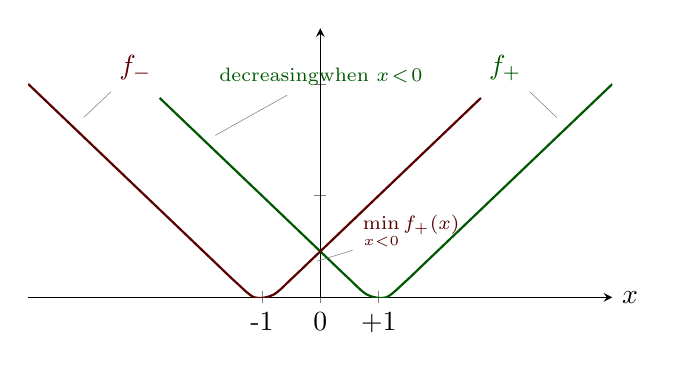
\begin{tikzpicture}
   \begin{axis}[width=9cm,height=5cm,
          %  grid = major,         
            axis y line=middle,
            axis x line=bottom,
						xlabel={$x$},
						every axis x label/.style={at={(current axis.right of origin)},anchor=west},
						%x label style={at={(4,-0.1)}},
						%ylabel={$f_v$},
           % grid style={dashed, gray!30},
            %xmin=-3,     % start the diagram at this x-coordinate
            %xmax=3,    % end   the diagram at this x-coordinate
						ymax=0.5,
						xtick={-1,0,1},
            xticklabels={-1,0,+1},
            yticklabels=\empty
            ]
           \addplot[domain=-2.75:5, green!35!black, thick,smooth] 
              {0.1*(x-1) + 2*0.01*ln(1+exp(-10*(x-1)))} node [pos=0.9,pin={135:$f_+$}] {} node [pos=0.1,pin={85:{\makecell{\scriptsize decreasing\\\scriptsize when $x\!<\!0$}}}] {}; 
            \addplot[domain=-5:2.75, red!35!black,thick,smooth] 
              {0.1*(x+1) + 2*0.01*ln(1+exp(-10*(x+1)))} node [pos=0.1,pin={45:$f_-$}] {} node [pos=0.615,pin={5:\makecell{\scriptsize$\min\limits_{x<0} f_+(x)$}}] {}; 
   \end{axis}
   \end{tikzpicture}}
	\caption{Plot of $f_+$ and $f_-$ with $\epsilon=0.1$}
\label{fig:lbfvdiff}
	  \end{subfigure}
	&
	  \begin{subfigure}[b]{0.5\textwidth}
 \centering
   \scalebox{0.8}{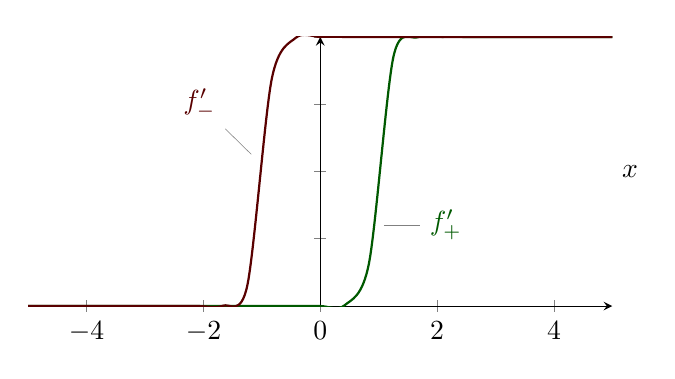
\begin{tikzpicture}
   \begin{axis}[width=9cm,height=5cm,
          %  grid = major,         
            axis y line=middle,
            axis x line=bottom,
						xlabel={$x$},
						every axis x label/.style={at={(current axis.right of origin)},anchor=west},
						%x label style={at={(4,-0.1)}},
						%ylabel={$f_v$},
           % grid style={dashed, gray!30},
            %xmin=-3,     % start the diagram at this x-coordinate
            %xmax=3,    % end   the diagram at this x-coordinate
						%xtick={-1,0,1},
            %xticklabels={-1,0,+1},
            yticklabels=\empty
            ]
           \addplot[domain=-5:5, green!35!black, thick,smooth] 
              {0.1*(1-exp(-10*(x-1)))/(1+exp(-10*(x-1)))} node [pos=0.59,pin={0:$f'_+$}] {}; 
            \addplot[domain=-5:5, red!35!black,thick,smooth] 
              {0.1*(1-exp(-10*(x+1)))/(1+exp(-10*(x+1)))} node [pos=0.4,pin={135:$f'_-$}] {}; 
							%\node at (axis cs:1,0.5) {P3};
   \end{axis}
   \end{tikzpicture}}
	\caption{Plot of $f'_+$ and $f'_-$ with $\epsilon=0.1$}
	\label{fig:fprime}
\end{subfigure}
	\end{tabular}
\end{figure}


Let $h(v) = -v + 2\epsilon\ln\dfrac{1+e^{\frac{v}{\epsilon}}}{2}$.
A simple algebra shows that $h$ is an even function, i.e., $h(v) = h(-v)$. Indeed,
\begin{align*}
h(v) = -v + 2\,\epsilon\,\ln\left(e^{\frac{v}{\epsilon}} \dfrac{1+e^{-\frac{v}{\epsilon}}}{2}\right)
= -v + 2\,\epsilon\, \dfrac{v}{\epsilon}  + 2\,\epsilon\,\ln\dfrac{1+e^{-\frac{v}{\epsilon}}}{2}
=  h(-v)\,.
\end{align*}
Specifically, $h(1) = h(-1)$ and thus
\begin{align*}
M = \epsilon\left(-1 + 2\epsilon\ln\dfrac{1+e^{\frac{1}{\epsilon}}}{2}\right)\,.
\end{align*}
From the foregoing, when $xv<0$, $\epsilon<\dfrac{1}{4\ln 2}$,  we have
\begin{align*}
f_v(x)-f_v(x_v^*) >\epsilon\left( -1 +2\epsilon \ln\dfrac{1+e^{\frac{1}{\epsilon}}}{2}  \right)> \dfrac{\epsilon}{2}.
\end{align*}
Hence,
%Using the fact that $f_+$ and $f_-$ are strongly convex with associated constant $\left(\dfrac{\epsilon}{2}\right)$, we obtain
\begin{align}
  f_v(x) - f_v(x^*_v)
  \ge \dfrac{\epsilon}{2}  \indic{x v  < 0}. \label{eq:fv-lb}
\end{align}
% Similarly,   $f_-(x) - f_-(x^*_-) \ge  \dfrac{\epsilon}{2}  \indic{x  >0}$.
We will consider the oracles $\gamma_v$ defined as 
\begin{align}
 \gamma_v(x,\delta) = \epsilon \,\dfrac{1-e^{-\frac{x-v}{\epsilon}}}{1+e^{-\frac{x-v}{\epsilon}}} - v\, \min(\epsilon,C_1 \delta^p) + \xi_\delta, \label{eq:main:oracle-1d}
\end{align}
where $\xi_\delta \sim \normal(0,\frac{C_2}{\delta^q})$.
% ; as with $f_v$, we will also use $\gamma_{+}$ ($\gamma_-$)  to denote $\gamma_{+1}$ (resp., $\gamma_{-1}$).
The oracle is indeed a $(c_1,c_2)$ Type-I oracle, with $c_1(\delta)=C_1\delta^p$ and $c_2(\delta)=\frac{C_2}{\delta^q}$.
%%%%%%%%%%%%%%%%%%%%%%%%%%%%%%%%%%%%%%%%%%%%%%%%%%%%%%%%%%%%%%%%%%%%%%%%%%%%%%% 

The minimax error \eqref{eq:minimaxerrdef} is lower bounded by
%\footnote{$f_{+1} \equiv f_+$ and $f_{-1}\equiv f_-$.}:
\begin{align}
\MoveEqLeft 
\Delta_n^{*} %\nonumber\\
  \ge  \inf_{\A} \,  \E[f_V(\hat X_n) - \inf_{x \in X}
  f_V(x)],\label{eq:avg-bd}
  \end{align}
where the expectation is w.r.t. the distribution $\P:= \dfrac{1}{2} \left(P_{\A, \gamma_+} \indic{v=+1} + P_{\A, \gamma_-}\indic{v=-1}\right)$ and $V: \Omega \to \{\pm 1 \}$ is defined by $V(g_{1:n},v) = v$.%
\footnote{Here, we are slightly abusing the notation as $\P$ depends on $\A$, but the dependence is suppressed.
In what follows, we will define several other distributions derived from $\P$, which will all depend on $\A$, but
for brevity this dependence will also be suppressed.
The point where the dependence on $\A$ is eliminated will be called to the reader's attention.}
%Here $\gamma_v$  is the oracle for $f_v$, for $v=+1,-1$ and is defined by $\gamma_v(x) = \epsilon(x-v) + v C_1 \delta^p$. 
Define $\P_{+}(\cdot) := \P(\cdot\mid V=1)$, $\P_{-}(\cdot) := \P(\cdot\mid
V=-1)$. 
% \todoa{This notation is somewhat confusing given the previous conventions.}
% \todoc{Better? I moved the definition upfront. I don't think there is much to complain about this definition. It is pretty clear.
% If you want, change it, but then do it consistently (and be . I have no time to change this and I have no idea what is that you would like.}
Using \eqref{eq:fv-lb}, we obtain
\begin{align}
\Delta_n^{*}  \ge & \inf_{\A} \dfrac{\epsilon}{2}\,  \P(\hat X_n V < 0), \label{eq:strong-convex-bd}\\
  = & \inf_{\A} \dfrac{\epsilon }{2} \, \left(\P_{+}(\hat X_n < 0) + \P_{-}(\hat X_n > 0)\right), \label{eq:Pplus}\\
  \ge &\inf_{\A} \dfrac{\epsilon }{2} \,\left(1 - \tvnorm{\P_{+}- \P_{-}}\right), \label{eq:lecam}\\
  \ge &\inf_{\A} \dfrac{\epsilon }{2}  \,\left( 1 - \left(\frac12\dkl{P_{+}}{P_{-}}\right)^{\frac{1}{2}}\right), \label{eq:pinsker}
\end{align}
where 
the equality in \eqref{eq:Pplus} uses the definitions of $\P_+$ and $\P_-$.  
Further, the inequality in \eqref{eq:lecam} follows from the definition of total variation distance, while \eqref{eq:pinsker} follows from Pinsker's inequality. %\todoc{You lost a factor of two here!}


%%%%%%%%%%%%%%%%%%%%%%%%%%%%%%%%%%%%%%%%%%%%%%%%%%%%%%%%%%%%%%%%%%%%%%%%%%%%%%% 
Define $G_t$ to be the $t$th observation of $\A$. Thus, $G_t:\Omega \to \R$, with $G_t( g_{1:n}, v) = g_t$.
Let $P_+^t(g_1,\dots,g_t)$ denote the joint distribution of $G_1,\dots,G_t$ conditioned on $V=+1$.
Let $P_{+}^t(\cdot\mid g_1,\ldots,g_{t-1})$ denote the distribution of $G_t$ conditional on $V=+1$ and $G_1=g_1,\ldots,G_{t-1}=g_{t-1}$. Define  $P_{-j}^t(\cdot\mid g_1,\ldots,g_{t-1})$ in a similar fashion.
Then, by the chain rule for KL-divergences, we have
\begin{align}
\label{eq:dklchain}
&\dkl{P_{+}}{P_{-}}= \sum_{t=1}^n \int_{\R^{t-1}} \dkl{P_{+}^t(\cdot\mid g_{1:t-1})}{P_{-}^t(\cdot\mid g_{1:t-1})} d P_{+}^t( g_{1:t-1}).
\end{align}
By the oracle's definition, $G_t \sim  \normal(\gamma_{+}(x^{\cA}_t(G_{1:t-1})),c_2(\delta^{\A}(G_{1:t-1})))$, i.e., 
$P_{+}^t(\cdot\mid g_{1:t-1})$ is the normal distribution with mean $\cA_t(g_{1:t-1})$ and variance $c_2(\delta^{\A}(G_{1:t-1}))$.
%, where $A(g_{1:t-1})$ denotes the point chosen by the algorithm given observations $g_1,\ldots, g_{t-1}$ and $\gamma_{+}$ is the gradient oracle defined earlier. 
Observe that, for any $x\in \R$, 
%$f_+'(x) - f_-'(x) = -2\epsilon$ and hence
\begin{align*}
0 \le f_-'(x) - f_+'(x) \le 2\,\epsilon \,\dfrac{e^{1/\epsilon}-1}{e^{1/\epsilon}+1} < 2\epsilon \,,
\end{align*}
cf. \cref{fig:fprime}.
Therefore,
\begin{align}
 |\gamma_+(x,\delta) - \gamma_-(x,\delta)| 
 = | f'_+(x) - \min(\epsilon,C_1 \delta^p - (f'_-(x)+\min(\epsilon,C_1 \delta^p)) | 
 < 2 (\epsilon - C_1 \delta^p)_+\,,
 \label{eq:gdiff-ub}
\end{align}
where $(u)_+ = \max(u,0)$ denotes the positive part of $u\in \R$.
%where $\delta(g_{1:t-1})$ is the tolerance parameter chosen by $\A$, based on the observations $g_{1:t-1}$. 
From the foregoing, using the abbreviations $x_t^{\A} = x^{\A}_t(g_{1:t-1})$ and $\delta_t^{\A} = \delta^{\A}_t(g_{1:t-1})$ (effectively fixing $g_{1:t-1}$ for this step),
\begin{align}
\dkl{P_{+}^t(\cdot\mid g_{1:t-1})}{P_{-}^t(\cdot\mid g_{1:t-1})}
& =\dfrac{(\gamma_{+}(x_t^{\A},\delta_t^{\A}) - \gamma_{-}(x_t^{\A},\delta_t^{\A}))^2}{2 c_2(\delta^{\A}_t)}
				\label{eq:dkgauss1}\\
& < \dfrac{2\{(\epsilon-C_1(\delta^{\A}_t)^p)_+\}^2\,(\delta^{\A}_t)^q}{C_2}\label{eq:dkgauss}\\
& \le  \sup_{\delta>0} \dfrac{2\{(\epsilon-C_1\delta^p)_+\}^2\,\delta^q}{C_2} \label{eq:supdelta}\,.
\end{align}
The equality \eqref{eq:dkgauss1} follows from the fact that the KL-divergence between normal distributions $\normal(\mu_1,\sigma^2)$ and $\normal(\mu_2,\sigma^2)$ is equal to $\dfrac{(\mu_1 - \mu_2)^2}{2 \sigma^2}$, while inequality \eqref{eq:dkgauss} follows from \eqref{eq:gdiff-ub}. Notice that the right-hand side of the above inequality does not depend on the algorithm anymore.

Now, observe that 
$\max_{\delta> 0} \{(\epsilon - C_1 \delta^p)_+\}^2 \delta^q = \max_{\delta> 0} (\epsilon - C_1 \delta^p)^2 \delta^q$. 
In other words, the maximizer $\delta_*$ of \eqref{eq:supdelta} can never be in the zero arm of the positive part 
function $(\epsilon - C_1 \delta^p)_+$,
and hence we maximize \eqref{eq:supdelta} by replacing the positive part with $(\epsilon - C_1 \delta^p)$ and imposing the condition $\epsilon/C_1 \ge \delta^p>0$.
Defining $z=p/q$, we obtain
\begin{align}
\delta_*=\left(\frac{\epsilon q}{2C_1(p+q/2)}\right)^{1/p} \text{ as long as }\epsilon<\frac{2z+1}{C_1^{2z-1}(z+1)^z}. \label{eq:deltastar}
\end{align}
\todoc[inline]{
I could not get this. 
I defined $u = \delta^q$, writing $(\epsilon-C_1 \delta^p)^2 \delta^q = (\epsilon-C_1 u^z)^2 u 
= \epsilon^2 u- 2C_1 \epsilon u^{z+1} + C_1^2 u^{2z+1}
= :f(u)$.
The first order optimality criterion is
$0 = f'(u) = C_1^2(2z+1) (u^z)^2 - 2 C_1 (z+1) \epsilon u^z + \epsilon^2$, from which I get
$(u^z)_{1,2} = \frac{2C_1(z+1)\epsilon \pm 2 C_1 z \epsilon}{2C_1^2(2z+1)}$.
I believe the minimizer is the larger of these two ($f$ first increases, then decreases, then increases).
From this, I get
$u^z = \epsilon/C_1$, and $\delta = (u^z)^{1/p} = (\epsilon/C_1)^{1/p}$.
I did not correct the rest besides minor editorial changes.}

Plugging \eqref{eq:supdelta} into \eqref{eq:dklchain}, we obtain
\begin{align}
\dkl{P_{+}}{P_{-}} \le \dfrac{2n}{C_2} (\epsilon-C_1\delta_*^p)_+^2 \delta_*^q.
\end{align}
Note that the above bound holds uniformly over all algorithms $\A$. 
Substituting the above bound into \eqref{eq:pinsker}, we obtain 
\begin{align}
 \Delta_n^{*}
  \ge & \dfrac{\epsilon}{2} \left(1 - \sqrt{
    n}  \dfrac{ (\epsilon-C_1\delta_*^p)_+\delta_*^{q/2}}{C_2}
  \right)\label{eq:final-lower-bd}
\end{align}

%%%%%%%%%%%%%%%%%%%%%%%%%%%%%%%%%%%%%%%%%%%%%%%%%%%%%%%%%%%%%%%%%%%%%%%%%%%%%%%
% \paragraph{Derivations of rates:}
%  Optimizing over $\epsilon$ in \eqref{eq:final-lower-bd}, we get
% $ \left(\dfrac{\delta^{-q/2}C_2}{4\sqrt{n}} + \dfrac{C_1\delta^p}{2}\right)$. We choose
% \[
% \epsilon^* = \left(\dfrac{\delta^{-q/2}C_2}{4\sqrt{n}} + C_1\delta^p\right)
% \]
% to guarantee that $\epsilon^*>C_1 \delta^p$.
% 
%  Plugging in $\epsilon^*$, we obtain
%  \[
%  \Delta_n^{*}
%  \ge \frac18 \left(\dfrac{\delta^{-q/2}C_2}{2\sqrt{n}} + C_1\delta^p \right).
%  \]
% 
% Substituting $p=1$ and $q=2$, we obtain
% \[
% \delta^*= \sqrt{\dfrac{C_2}{2C_1}}\dfrac{1}{n^{\frac{1}{4}}} \text{ and } 
% \Delta_n^{*} \ge \left(\dfrac{\sqrt{2C_1C_2}}{4}\right)\dfrac{1}{n^{\frac{1}{4}}}.
% \]
% 
% On the other hand, substituting $p=q=2$, we obtain
% \[
% \delta^*= \left(\dfrac{C_2}{2C_1}\right)^{\frac{1}{3}}\dfrac{1}{n^{\frac{1}{6}}} \text{ and } \Delta_n^{*} \ge \left(\dfrac{C_1^{\frac{1}{3}}C_2^{\frac{2}{3}}}{4\, 2^{\frac{1}{3}}}\right)\dfrac{1}{n^{\frac{1}{3}}}.
% \]

\paragraph{Derivation of the rates uniformly for all $\delta$:}

The condition on $\epsilon$ above can be inferred from the constraint $\epsilon/C_1 \ge {\delta^*}^p$.

From the foregoing, we have the following lower bound on the minimax error $\Delta_n^{(1)*}$:
\[
\Delta_n^{(1)*} \ge \dfrac{\epsilon}{2} \left(1 - \sqrt{n}  \dfrac{K_1}{2+\frac{q}{2p}} \epsilon^{\frac{p+\tfrac{q}{2}}{p}}\right), \text{ where } K_1 = \dfrac{4p+q}{\sqrt{C_2}(p+\tfrac{q}{2})} \left(\dfrac{q}{2C_1(p+\tfrac{q}{2})}\right)^{\frac{q}{2p}}.
\]
 
Plugging in $\epsilon = \left(\dfrac{1}{\sqrt{n} K_1} \right)^{\frac{p}{p+\frac{q}{2}}}$, we see that the conditions on $\epsilon$ are satisfied for large enough $n$, and for such $n$ we obtain
\begin{align}
\Delta_n^{(1)*} \ge \dfrac{2p+q}{8p+2q}\left(\dfrac{1}{ K_1 \sqrt n}\right)^{\frac{p}{p+\frac{q}{2}}}.
\label{eq:lb-pq}
\end{align}
The conditions on $n$ for the above bound to hold are:
\begin{align}
\frac{1}{\sqrt{d}}\left(\frac{1}{\sqrt{n} K_1} \right)^{\frac{p}{p+\frac{q}{2}}}\le \min\left( \frac{C_1 (2p+q)}{q}, \frac{2z+1}{C_1^{2z-1}(z+1)^z}\right).
\end{align}
The above conditions on $n$ can be inferred from (i) the requirement on  $\epsilon$ in \eqref{eq:deltastar}, (ii) assumption $\delta \le 1$ in Definition \ref{def:oracle1},  and (iii) the optimal choice of $\epsilon$ above.

Now, when $q=2$ and $p=1$, the lower bound in \eqref{eq:lb-pq} simplifies to
\[
\Delta_n^{(1)*} \ge \dfrac{ (4C_1^2C_2)^{1/4}}{3\sqrt{3}} n^{-1/4}, \text{ for } \epsilon=\sqrt{2/3}C_1^{1/2}C_2^{1/4} n^{-1/4}.
\]
On the other hand, for $p=q=2$, we obtain
\[
\Delta_n^{(1)*} \ge  \frac{9}{10}\left(\frac{C_1 C_2}{100}\right)^{1/3} n^{-1/3} \text{ for } \epsilon=3\left(\frac{C_1 C_2}{100}\right)^{1/3}n^{-1/3}.
\]



%%%%%%%%%%%%%%%%%%%%%%%%%%%%%%%%%%%%%%%%%%%%%%%%%%%%%%%%%%%%%%%%%%%%%%%%%%%%%%%
%%%%%%%%%%%%%%%%%%%%%%%%%%%%%%%%%%%%%%%%%%%%%%%%%%%%%%%%%%%%%%%%%%%%%%%%%%%%%%%
%%%%%%%%%%%%%%%%%%%%%%%%%%%%%%%%%%%%%%%%%%%%%%%%%%%%%%%%%%%%%%%%%%%%%%%%%%%%%%%
\paragraph{Generalization to $d$ dimensions:}

Let $\cK \subset \R^d$.
Define $f_v$ for any $v\in \{-1,+1\}^d$ as follows: For any $x \in \cK$, 
\begin{align*}
  f_v(x) :=& \sum_{i=1}^d f^{(i)}_{v_i}(x_i), \,\,  \text{ where }
  f^{(i)}_{v_i}(x_i) := \epsilon\left( x_i-v_i\right)+2\epsilon^2 \ln\left(1+e^{-\frac{x_i-v_i}{\epsilon}}  \right),  \,\, \text{ for } i=1,\ldots,d.
\end{align*}
By definition, $f_v$ is additively separable and minimized at $x^*_v=v$ with the minimum value being zero.
We consider oracles $\gamma_v$ defined by
$\gamma_v(x) = \sum_{i=1}^d \gamma_{v_i}^{(i)}e_i$, where 
$e_i$ is the $i$th unit vector in the standard Euclidean base,
$\gamma_{v_i}^{(i)} = 
\epsilon \dfrac{1-e^{-\frac{x_i-v_i}{\epsilon}}}{1+e^{-\frac{x_i-v_i}{\epsilon}}} - v\, \frac{C_1 \delta^p}{\sqrt{d}}  + \xi_i
$, where $\xi_i \sim \normal(0,\frac{C_2}{d\delta^q})$. 
It is evident that the $\gamma$ is a $(c_1,c_2)$ Type-I oracle, with $c_1(\delta)=C_1\delta^p$ and $c_2(\delta)=\frac{C_2}{\delta^q}$.

Let $\Delta_n^{(d)*}$ denote the minimax error $\Delta_n^*\left(\F_d, C_1\delta^p,\frac{C_2}{\delta^q}\right)$ for the $d$-dimensional family of functions $\F_d$, which is composed of $f_v$s, as defined above. We have
\begin{align*}
 \Delta_n^{(d)*} \ge& \inf_\A  \sup_{v\in \{\pm 1 \}^d}\sum_{i=1}^d L_i(v), \text{ where, for } i=1,\ldots,d,\\
 L_i(v) := & \int f^{(i)}_{v_i}(\hat X_{ni}(g_{1:n}) )\, dP_{\A,\gamma_v,\sigma^2}(g_{1:n}),  
\end{align*}
where $\hat{X}_{ni}$ denotes the $i$th coordinate of the vector $\hat{X}_n \in \R^d$ chosen by $\A$, for $i=1,\ldots,d$
(again, to simplify the notation the dependence of $\hat{X}_n$ on $\A$ is suppressed).


% Fix an $i$ and consider the loss $L_i(v)$.
% We now argue that, since $f_v$ is separable, any algorithm $\A$ that uses information in dimensions other than $i$ in the gradient samples of the oracle, can be replaced by $d$ algorithms $\A_1^*$, $\dots$, $\A_d^*$ such that $\A_i^*$ is only using information for dimension $i$ and is only predicting the $i$th coordinate at the end, and the sum of losses they incur is utmost that of $\A$ in the worst-case.

\begin{lemma}
\label{lemma:sep}
For any algorithm $\A$, there exist  $d$ ``$1$-dimensional'' algorithms, $\A_i^*$, $1\le i \le d$,
the $i$th algorithm interacting with only a one dimensional oracle, supplying gradient estimates about $f_{v_i}^{(i)}$ 
such that if $L^{\A}(v)$ is the loss of $\A$ on environment with index $v$ and the following holds
the 
\begin{align}
\label{eq:onedimlb}
% \begin{split}
% \MoveEqLeft 
&\max_{v\in \{\pm 1\}^d} L^{\A}(v) 
\ge   \max_{v_1\in \{\pm 1\}} L_1^{\A_1^*}(v_1) + \dots + \max_{v_d\in \{\pm 1 \}} L_d^{\A^*_d}(v_d)\,.
% \end{split}
\end{align}
\end{lemma}
\begin{proof}
Let $v_{-i}=(v_1,\ldots,v_{i-1},v_{i+1},\ldots,v_d)$ denote a $d-1$ dimensional vector that removes the $i$th coordinate from $v$. By an abuse of notation, we let $v=(v_i, v_{-i})$. 
We now describe the construction of $\A^*=(\A_1^*, \ldots, \A_d^*)$.
We describe $\A_1^*$ only, other algorithm components are formed in a similar manner.

To define $\A_1^*$, consider the solution of the following max-min problem:
\[
\max_{v_1} \min_{v_{-1}} L_1(v_1, v_{-1})).
\]
Let the optimal solution of this problem be denoted by $(\hat{v}_1^*,v_{-1}^*)$.
The algorithm will make use of $v_{-1}^*$ (which it does have access to) in the following manner:
Recall that $L$ and $L_1$ are defined as a function of $(\gamma_v)_{v\in \{\pm\}^d}$.
Let $v\in \{\pm 1\}^d$ be fixed, unknown to $\A$ and $\A_1^*$. 
The algorithm construction will make use of $\gamma_v$ and $\gamma_{(1,v_{-1}^*)}$ in the following manner:
At time $t=1$, $\A_1^*$ consults $\A$ to get $\delta$ and the point $X_1\in \cK$.
Next, it asks the oracle $\gamma_v$ for a $d$ dimensional gradient estimate of $f_v$ at $X_1$ with tolerance $\delta$,
obtaining $G_1'$.
At the same time, it also asks $\gamma_{(1,v_{-1}^*)}$ for another $d$ dimensional gradient estimate (this has nothing to do with $f_v$), obtaining $G_1''$.
Then, $G_1 = (G_{1,1}',G_{1,-1}'')$ is fed to $\A$, which returns $X_2\in \cK$. From this point up to the end the process is similar: Both oracles are queried and the gradient to be fed to $\A$ is synthetized by putting together the first component of the gradient estimate from $\gamma_v$ and the last $d-1$ components obtained from $\gamma_{(1,v_{-1}^*)}$.
Finally, at the end, $\A$ produces $\hat{X}_n$, and $\A_1^*$ returns $\hat{X}_{n,1}$.
Clearly, by construction and the definition of $L_1$,
the expected loss $L^*_1(v_1)$ of $\A_1^*$ on $f_{v_1}^{(1)}$ is $L_1(v_1,v_{-1}^*)$, while $\A_1^*$ only uses the first coordinates of the gradients that it gets from the oracle $\gamma_v$.
With similar definitions, $L^*_i(v_i)$, the expected loss of $\A_i^*$ on $f_{v_i}^{(i)}$ is $L_i(v_i,v_{-i}^*)$, $2\le i \le d$.
Now, notice that $L_i(\hat{v}_i^*,v_{-i}^*) = \min_{v_{-i} } L_i(\hat{v}_i^*,v_{-i}) \le L_i(\hat{v}_i^*, \hat{v}_{-i}^*)$,
where $\hat{v}_{-i}^*$ is the vector obtained by discarding the $i$th component of $\hat{v}^* = (\hat{v}_1^*,\dots,\hat{v}_d^*)$.
Thus,
\begin{align*}
&\max_{v\in \{\pm 1 \}^d }
L^*_1(v_1) + \dots + L^*_d(v_d) \\
&   = \max_{v\in \{\pm 1 \}^d } L_1(v_1,v_{-1}^*) + \dots + L_d(v_d,v_{-d}^*)\\
& = \max_{v_1\in \{\pm 1\}} L_1(v_1,v_{-1}^*) + \dots +  \max_{v_d\in \{\pm 1\}} L_d(v_d,v_{-d}^*)\\
& = L_1(\hat{v}^*_1,v_{-1}^*) + \dots +   L_d(\hat{v}^*_d,v_{-d}^*)\\
& \le L_1(\hat{v}^*_1,\hat{v}_{-1}^*) + \dots +  L_d(\hat{v}^*_d,\hat{v}_{-d}^*)\\
& \le L(\hat{v}^*) \le \max_{v\in \{\pm 1\}^d } L(v)\,,
\end{align*}
which was the claim to be proven.
\end{proof}

\paragraph{Main proof:}
The minimax error $\Delta_n^{(d)*}$ can be lower bounded as follows:
\begin{align}
\Delta_n^{(d)*}  &\ge  \inf_{\A} \max_{v\in {\pm 1}^d} L^\A(v) \nonumber\\
 & \ge \inf_{\A_1} \max_{v_1\in \{\pm 1\}} L_1^{\A_1}(v_1) + \dots + 
 			\inf_{A_d} \max_{v_d\in \{\pm 1 \}} L_d^{\A_d}(v_d) \label{eq:splitA}\\
%             \ge & \inf_{\A_1^*} L_1(v^*) + \ldots + \inf_{\A_d^*} L_d(v^*) \label{eq:splitA}\\
               & \ge d \Delta_n^{*}\left(\F_1,\frac{C_1\delta^p}{\sqrt d}, \frac{C_2}{d\delta^q}\right)\,, \label{eq:dlb}
\end{align}
where in inequality \eqref{eq:splitA}, algorithms $\A_i$ are interacting with the respective one-dimensional oracles $\gamma^{(i)}_{v_i}$ only 
and the inequality follows by~\eqref{eq:onedimlb},
while the inequality \eqref{eq:dlb} follows from the fact that each infimum term in \eqref{eq:splitA} is solving a $1$-dimensional problem and hence the bound in \eqref{eq:final-lower-bd} applies with $C_1$ replaced by $C_1/\sqrt{d}$ and $C_2$ replaced by $C_2/d$. The resulting bound is denoted by $\Delta_n^{*}\left(\F_1,\frac{C_1\delta^p}{\sqrt d}, \frac{C_2}{d\delta^q}\right)$. 
% is the one-dimensional minimax error, which is lower-bounded in \eqref{eq:final-lower-bd}. \todoc{However, I would have written just the $1$d final bound there, or $\Delta_n^*( \dots )$ with some notation, because we don't want to redo this whole optimization business..}

% Using the one-dimensional minimax error $\Delta_n^{*}$, we obtain
% \[\Delta_n^* \ge d \Delta_n^{*}.\]
\paragraph{Derivation of rates:}\ \\
Plugging the bound derived in \eqref{eq:lb-pq} for $1$-dimensional setting into the bound in \eqref{eq:dlb}, we obtain the following result for any $p, q >0$:
\begin{align}
\Delta_n^{(d)*} \ge  \dfrac{2p+q}{8p+2q}\sqrt{d}\left(\dfrac{1}{ K_1 \sqrt n}\right)^{\frac{p}{p+\frac{q}{2}}} \text{ for } 
\epsilon = \dfrac{1}{\sqrt{d}}\left(\dfrac{1}{\sqrt{n} K_1} \right)^{\frac{p}{p+\frac{q}{2}}}.
\label{eq:lb-pq-d}
\end{align}

The above bound simplifies to the following for the case where $p=1$ and $q=2$:
\begin{align*}
% \Delta_n^{*}\left(\F_1,\frac{C_1\delta^p}{\sqrt d}, \frac{C_2}{d\delta^q}\right) \ge &\frac{1}{2}\sqrt{\frac{C_1 C_2}{2 d^{\frac{3}{2}}}} n^{-1/4} \text{ and hence,} \\
\Delta_n^{(d)*}  \ge& \dfrac{ (4C_1^2C_2)^{1/4}}{3\sqrt{3}} d^{1/2}n^{-1/4}.
\end{align*}

On the other hand, for the case $p=q=2$, we obtain
\begin{align*}
% \Delta_n^{*}\left(\F_1,\frac{C_1\delta^p}{\sqrt d}, \frac{C_2}{d\delta^q}\right) \ge &\dfrac{3}{8}\left(\frac{C_1 C_2^2}{16 d^{\frac{5}{2}}}\right)^{1/3} n^{-1/3} \text{ and hence,} \\
\Delta_n^{(d)*}  \ge& \frac{9}{10}\left(\frac{C_1 C_2}{100}\right)^{1/3} d^{1/2}n^{-1/3}.
\end{align*}
%%% Local Variables: 
%%% mode: latex
%%% TeX-master: "bgo"
%%% End: 

\subsection{Proof of Theorem \ref{thm:lb-convex} for strongly convex + smooth function class $\F_{L,1}(\K)$}
\label{sec:appendix-lbscconvex}
We follow the notational convention used earlier for convex functions in one dimension. 
\todoc{This proof needs to be updated to allow the algorithm choose $\delta$, the same way, as was done for the smooth case.
The oracle also takes two parameters, as there, etc.
In general, this text is too rough (typos, etc.).
Read the other proof carefully and change this proof to reflect closely the other one. Don't make it longer, just correct the slight imprecisions.}

We consider functions $f_v$, for any $v \in \{-\nu,+\nu\}$, defined as
By assumption,  $\{f_+, f_-\}\subset \F$, with 
\begin{align*}
  f_v(x) := \dfrac{1}{2} x^2 - v x \,\, x \in \cK\,;
\end{align*}
we will slightly abuse notation by using $f_+$ ($f_-$) in place of $f_{+\nu}$ (resp., $f_{-\nu}$).
%%%%%%%%%%%%%%%%%%%%%%%%%%%%%%%%%%%%%%%%%%%%%%%%%%%%%%%%%%%%%%%%%%%%%%%%%%%%%%% 

Clearly, $f_v$ is minimized at $x^*_v = v$.
By the definition of $f_v$, we have
%Using the fact that $f_+$ and $f_-$ are strongly convex with associated constant $\left(\dfrac{\epsilon}{2}\right)$, we obtain
\begin{align}
  f_v(x) - f_v(x^*_v)
\ge  \dfrac{\nu^2}{2}  \indic{x v  < 0}. \label{eq:fv-lb-sc}
\end{align}
We will consider the oracles $\gamma_v$ defined as 
\begin{align}
 \gamma_v(x) = \epsilon(x-v) - \sign(v)\, \min(v,C_1 \delta^p) + \xi, \label{eq:oracle-1d}
\end{align}
where $\xi \sim \normal(0,\frac{C_2}{\delta^q})$; as with $f_v$, we will also use $\gamma_{+}$ ($\gamma_-$) 
to denote $\gamma_{+1}$ (resp., $\gamma_{-1}$).
The oracle is indeed a $(c_1,c_2)$ Type-I oracle, with $c_1(\delta)=C_1\delta^p$ and $c_2(\delta)=\frac{C_2}{\delta^q}$.
%%%%%%%%%%%%%%%%%%%%%%%%%%%%%%%%%%%%%%%%%%%%%%%%%%%%%%%%%%%%%%%%%%%%%%%%%%%%%%% 

Using arguments similar to those in the proof of lower bound for convex functions, we obtain
\begin{align}
\Delta_n^{*} %\nonumber\\
  \ge  &\inf_{\A} \dfrac{\epsilon }{2}  \,\left( 1 - \left(\frac12\dkl{P_{+}}{P_{-}}\right)^{\frac{1}{2}}\right), \label{eq:pinskersc}
\end{align}
Note that $P_+$ (resp. $P_-$) is $\P$ conditioned on the event $V=+\nu$ (resp. $V=-\nu$), since $v$ takes values in $\{+\nu,-\nu\}$. The conditioning in the earlier proof for convex function was on $V=+1$ for $P_+$ as $v$ there was taking values $\{+1,-1\}$.
%%%%%%%%%%%%%%%%%%%%%%%%%%%%%%%%%%%%%%%%%%%%%%%%%%%%%%%%%%%%%%%%%%%%%%%%%%%%%%% 

Observe that, for any $x\in \R$, $f_+'(x) - f_-'(x) = 2v$ and hence
\begin{align}
 |\gamma_+(x) - \gamma_-(x)| 
& = | f'_+(x) - \min(v,C_1 \delta^p) - (f'_-(x)+\min(v,C_1 \delta^p)) | \nonumber \\
& = 2 (\nu - C_1 \delta^p)_+.
 \label{eq:gdiff-ub-sc}
\end{align}
From the foregoing, 
\begin{align}
 \MoveEqLeft \dkl{P_{+}^t(\cdot\mid g_{1:t-1})}{P_{-}^t(\cdot\mid g_{1:t-1})}\nonumber\\
 \le & \dfrac{2(\nu-C_1\delta^p)_+^2\delta^q}{C_2},\label{eq:dkgausssc}
\end{align}
where the inequality \eqref{eq:dkgausssc} follows from \eqref{eq:gdiff-ub-sc}.
Thus, we obtain
\begin{align}
\dkl{P_{+}}{P_{-}} \le \dfrac{2n(\nu-C_1\delta^p)_+^2 \delta^q}{C_2}.
\end{align}
Substituting the above bound into \eqref{eq:pinskersc}, we obtain 
\begin{align}
 \Delta_n^{*}
  \ge & \dfrac{\nu^2}{2} \left(1 - \sqrt{
    n}  \dfrac{(\nu-C_1\delta^p)_+\delta^{q/2}}{C_2}
  \right)\label{eq:final-lower-bd-sc}
\end{align}


\paragraph{Derivation of the rates uniformly for all $\delta$:}
As in the proof of the lower bound for $\F_{L,0}(\K)$, we replace the positive part function in \eqref{eq:final-lower-bd-sc} and optimize over $\delta$ to obtain the following:
\begin{align}
\delta^*=\left(\frac{\nu q}{2C_1(p+q/2)}\right)^{1/p} \text{ as long as }\nu<\frac{2z+1}{C_1^{2z-1}(z+1)^z},
\label{eq:deltastar-sc}
\end{align}
where $z=p/q$. Recall that we require $\nu/C_1 \ge {\delta^*}^p$, which results in the condition on $\nu$ above.

From the above, we have the following lower bound for the minimax error $\Delta_n^{(1)*}$ for any choice of $\delta$:
% and for any choice of $\delta$, the minimax error $\Delta_n^{*}$ satisfies
\[
\Delta_n^{(1)*} \ge \dfrac{\nu^2}{2} \left(1 - \sqrt{n}  K_1 \nu^{\frac{p+\tfrac{q}{2}}{p}}\right), \text{ where } K_1 = \dfrac{p}{C_2(p+\tfrac{q}{2})} \left(\dfrac{q}{2C_1(p+\tfrac{q}{2})}\right)^{\frac{q}{2p}}.
\]


Plugging in $\nu = \left(\dfrac{1}{2\sqrt{n} K_1} \right)^{\frac{p}{p+\frac{q}{2}}}$, we obtain
\begin{align}
\Delta_n^{(1)*} \ge \dfrac{1}{4}\left(\dfrac{1}{2 K_1 \sqrt n}\right)^{\frac{2p}{p+\frac{q}{2}}}.
\label{eq:lb-pq-sc}
\end{align}
The above bound holds for $n$ such that 
$$\!d^{\frac{-(4p+q)}{(2p+q)}}\!\!\left(\frac{1}{2\sqrt{n} K_1} \right)^{\!\!\frac{p}{p+\frac{q}{2}}} \!\!\!\le \!\!\min\!\left( \frac{C_1 (2p+q)}{q}, \frac{2z+1}{C_1^{2z-1}(z+1)^z}\!\right).$$
As in the proof of the lower bound for $\F_{L,0}(\K)$, the first condition on $n$ above is due to the assumption that $\delta \le 1$ in Definition \ref{def:oracle1}, while the second condition is due to the constraint on $\nu$ in \eqref{eq:deltastar-sc}.

Now, when $q=2$ and $p=1$, the lower bound in \eqref{eq:lb-pq-sc} simplifies to
\[
\Delta_n^{(1)*} \ge \dfrac{C_1 C_2}{2} n^{-1/2}, \text{ for } \nu = 2C_1C_2 n^{-1/2}.
\]
On the other hand, for $p=q=2$, we obtain
\[
\Delta_n^{(1)*} \ge  \frac{9}{4}\left(\frac{C_1 C_2^2}{16}\right)^{1/3} n^{-2/3} \text{ for } \nu=\frac{9}{2}\left(\frac{C_1 C_2^2}{16}\right)^{1/3}n^{-2/3}.
\]


%%%%%%%%%%%%%%%%%%%%%%%%%%%%%%%%%%%%%%%%%%%%%%%%%%%%%%%%%%%%%%%%%%%%%%%%%%%%%%%
%%%%%%%%%%%%%%%%%%%%%%%%%%%%%%%%%%%%%%%%%%%%%%%%%%%%%%%%%%%%%%%%%%%%%%%%%%%%%%%

\paragraph{Generalization to $d$ dimensions:}
The proof in $d$ dimensions for strongly convex functions follows in similar fashion as that for the case of convex functions and we obtain the following rates:\\
General $p, q >0$:
\begin{align}
\Delta_n^{(d)*} \ge \dfrac{1}{4} d^{\frac{-2p}{(2p+q)}} \left(\dfrac{1}{2 K_1 \sqrt n}\right)^{\frac{2p}{p+\frac{q}{2}}} \text{ for } 
\nu = d^{\frac{-(4p+q)}{(2p+q)}}\left(\dfrac{1}{2\sqrt{n} K_1} \right)^{\frac{p}{p+\frac{q}{2}}}.
\label{eq:lb-pq-d}
\end{align}

Case $p=1$ and $q=2$:
\begin{align*}
% \Delta_n^{*}\left(\F_1,\frac{C_1\delta^p}{\sqrt d}, \frac{C_2}{d\delta^q}\right) \ge &\frac{1}{2}\sqrt{\frac{C_1 C_2}{2 d^{\frac{3}{2}}}} n^{-1/4} \text{ and hence,} \\
\Delta_n^{(d)*}  \ge& \dfrac{C_1 C_2}{2} n^{-1/2} d^{-1/2}.
\end{align*}

Case $p=q=2$:
\begin{align*}
% \Delta_n^{*}\left(\F_1,\frac{C_1\delta^p}{\sqrt d}, \frac{C_2}{d\delta^q}\right) \ge &\dfrac{3}{8}\left(\frac{C_1 C_2^2}{16 d^{\frac{5}{2}}}\right)^{1/3} n^{-1/3} \text{ and hence,} \\
\Delta_n^{(d)*}  \ge& \frac{9}{4}\left(\frac{C_1^2 C_2^4}{16}\right)^{1/3} n^{-2/3} d^{-2/3}.
\end{align*}
